%----------------------------------------------------
% Setup Beamer
%----------------------------------------------------
\documentclass[hyperref={colorlinks=true}]{beamer}

%----------------------------------------------------
% Packages to use
%----------------------------------------------------
\input{../packages.sty}

%----------------------------------------------------
% Setup Theme
%----------------------------------------------------
\input{../theme.sty}

%----------------------------------------------------
% Table of Contents at each section transition
%----------------------------------------------------

\AtBeginSection[]
{
   \begin{frame}
       \frametitle{Outline}
       \setcounter{tocdepth}{2}
       \tableofcontents[currentsection]
   \end{frame}
}

%----------------------------------------------------
% Colors
%----------------------------------------------------
\input{../mycolors.sty}

%----------------------------------------------------
% Style, formatting, and new commands
%----------------------------------------------------
\input{../../global.sty}
\input{../newcommands.sty}
\input{../EandMcommands.sty}

%----------------------------------------------------
% Set paths for plots and images
%----------------------------------------------------
\input{../paths.sty}

%----------------------------------------------------
% SETTINGS FOR THIS LECTURE
%----------------------------------------------------
\newcommand{\lecnum }  {Lecture 11}
\newcommand{\lecdate}  {November 5, 2019}
\newcommand{\topic}    {Fourier Transforms!}

%-----------------------------------------------------------------------------------------
% Title: [Column]{Title}
%-----------------------------------------------------------------------------------------
\title[PHYS 250 (Autumn 2019) -- \lecnum]{\topic}

%-----------------------------------------------------------------------------------------
% SubTitle: [Column]{Subtitle}
%-----------------------------------------------------------------------------------------
\subtitle{PHYS 250 (Autumn 2019) -- \lecnum}

%-----------------------------------------------------------------------------------------
% Author: [SubAuthor]{Author}
%-----------------------------------------------------------------------------------------
\author[D.W.~Miller]{David Miller}

%----------------------------------------------------
% Institute: [SubInst]{Institute}
%----------------------------------------------------
\institute[EFI, Chicago] 
{
  Department of Physics and the Enrico Fermi Institute\\
  University of Chicago
}

%----------------------------------------------------
% Institute: [SubInst]{Institute}
%----------------------------------------------------
\date[\lecdate]{\lecdate}

\subject{PHYS 250 Lecture}

\begin{document}

%==========================================================================================
% TITLE PAGE
%==========================================================================================

{
\begin{frame}
  \titlepage
\end{frame}
}

%==========================================================================================
\section[Plan going forward]{Plan going forward}
%==========================================================================================

%-----------------------------------------------------------------------------------------
\subsection[Data analysis tools]{Data analysis tools}
%-----------------------------------------------------------------------------------------

\begin{frame}%[shrink=10]
  \frametitle{Moving towards physics data analysis}

  As we discussed last time, I would like to take the direction of this quarter more towards practical physics data analysis and algorithms. We will start with \textbf{Fourier Transforms} and \textbf{Neural Networks} and then analyze data from the \bluebf{CMB, LIGO, and/or the Large Hadron Collider}.
  
  \vspace{0.3cm}
  
  \begin{ucblock}{Fourier Analysis and Neural Networks}
    \begin{itemize}
      \item \bluebf{Fourier Series and Analysis:} 
      \begin{itemize}
        \item Discussing the basics of Fourier Series 
        \item Evaluate, computationally, the coefficients of a simple series for both a square and sawtooth wave
        \item Extend discussion to the \alertbf{Fast Fourier Transform}
      \end{itemize}
      \item \bluebf{Neural Networks:} 
      \begin{itemize}
        \item Training computers to discover, identify, and analyze patterns of interest in datasets 
        \item Modeling perspective on what a neural network achieves
        \item Structure and function of a neuron
        \item Mathematical properties of a neural network
      \end{itemize}
    \end{itemize}
  \end{ucblock}
  
  \mysp
  
  This will be a mixture of Python Notebooks and Lecture Slides

\end{frame}


%==========================================================================================
\section[The Square Wave]{The Square Wave}
%==========================================================================================

%-----------------------------------------------------------------------------------------
\subsection[Square Wave]{Square Wave}
%-----------------------------------------------------------------------------------------

\begin{frame}%[shrink=10]
  \frametitle{Square Wave}

  Let's start with the Fourier Series for the \alertbf{square wave} function.
  
  \mysp
  
  As you may have heard in a variety of contexts (e.g. PHYS 133!) we can decompose any periodic function or periodic signal into the weighted sum of a (possibly infinite) set of simple oscillating functions, namely sines and cosines (or, equivalently, complex exponentials). 

  \begin{equation}
    f(x) = \frac{a_0}{2} + \sum_{n=1}^{\infty} a_n \cos(nx) + b_n \sin(nx)
  \end{equation}

This is possible because the trigonometric functions for a \alertbf{set of complete, orthogonal basis vectors} that span the space.

  \mysp

  \centering \bluebf{Now open up the \texttt{Fourier-Series.ipynb} jupyter notebook and we will discuss this more deeply!}


\end{frame}
  
%-----------------------------------------------------------------------------------------

\begin{frame}
  \frametitle{Fourier series for a square wave}
    
  We may determine the coefficients of a sine and cosine expansion to be:
  
  \begin{equation}
    a_n =\frac{2}{n\pi}\sin \left(n \omega_0 \frac{\pi}{2} \right)
  \end{equation}
  
  which yields a discrete function:
  
  \begin{equation}
    f(x) = \frac{a_0}{2} + \sum_{n=1}^{\infty} a_n \cos(nx) 
  \end{equation}
  
  \centering \bluebf{Now open up the \texttt{Fourier-Transforms-Analysis.ipynb} jupyter notebook so that we can look at this in more detail!}

\end{frame}

%==========================================================================================
\section[Extension to the Fourier Transform]{Extension to the Fourier Transform}
%==========================================================================================

%-----------------------------------------------------------------------------------------
\subsection[Euler's Formula]{Euler's Formula}
%-----------------------------------------------------------------------------------------


\begin{frame}%[fragile]
  \frametitle{Euler's Formula}

  We can generalize this by making use of Euler's Formula.
  
  \begin{columns}
  
  \column{0.5\textwidth}
  
  Euler's formula states that for any real number $\phi$: 
  
  \begin{equation}
    e^{i\phi} = \cos(\phi) + i\sin(\phi)
  \end{equation}
  
  When $\phi=\pi$, Euler's formula evaluates to 
  
  \begin{equation}
    e^{i\pi }+1=0,
  \end{equation} 
  
  which is known as Euler's identity. 
  
  \column{0.5\textwidth}
  
  \begin{figure}
    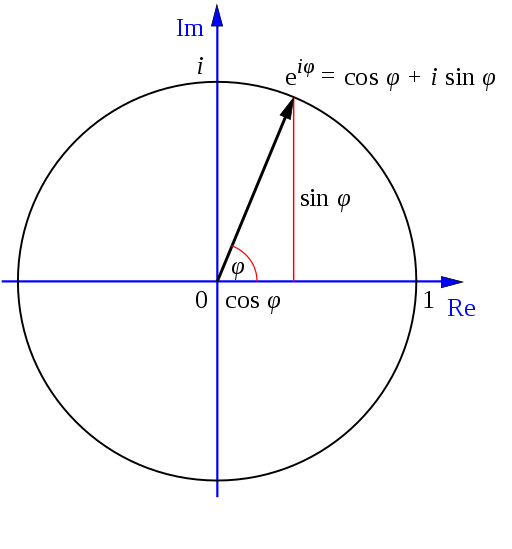
\includegraphics[width=0.9\columnwidth]{Eulers_formula.png}
  \end{figure}
  
  \end{columns}
  
  The implication is that it is possible to recover the amplitude of each wave in a Fourier series using an integral, which has many useful properties (in particular, that it's then continuous).

\end{frame}

%-----------------------------------------------------------------------------------------
\subsection[Fourier Transforms]{Fourier Transforms}
%-----------------------------------------------------------------------------------------

\begin{frame}%[fragile,shrink=15]
  \frametitle{Fourier Transforms (I)}

  I will use the following definitions for the Fourier transform $\hat{f}(\xi)$ of a function $f(x)$, where $x$ typically represents either a \bluebf{spatial or time domain}, and $\xi$ typically represents a corresponding inverse notion of \alertbf{spatial or time frequency}.

  \begin{equation}
    \hat{f}(\xi)=\int_{-\infty}^{\infty} f(x) e^{-2\pi i \xi x } dx
  \end{equation}
  
  The \alertbf{inverse transform} is then obtained via
  
  \begin{equation}
    f(x)=\int_{-\infty}^{\infty} \hat{f}(\xi) e^{2\pi i \xi x } d\xi 
  \end{equation}

  In the case of spatial coordinates, $x$ denotes length and $\xi$ denotes inverse wavelength: $\xi = \frac{1}{\lambda}$. In the time domain, $x$ denotes time and $\xi$ denotes frequency. In the case that $x=t$ is in seconds, but $\xi$ is \alertbf{angular} frequency $\omega$ then a factor of $2\pi$ appears to get the normalization correct.

\end{frame}

%-----------------------------------------------------------------------------------------

\begin{frame}%[fragile,shrink=15]
  \frametitle{Fourier Transforms (II)}

  In the case of spatial coordinates, $x$ denotes length and $\xi$ denotes inverse wavelength: $\xi = \frac{1}{\lambda}$. In the time domain, $x$ denotes time and $\xi$ denotes frequency. In the case that $x=t$ is in seconds, but $\xi$ is \alertbf{angular} frequency $\omega$ then a factor of $2\pi$ appears to get the normalization correct.
  
  \begin{eqnarray}
    \hat{f}(\omega) &=& \frac{1}{\sqrt{2\pi}} \int_{-\infty}^{\infty} f(t) e^{-i\omega t} dt \\
    f(t)            &=& \frac{1}{\sqrt{2\pi}} \int_{-\infty}^{\infty} \hat{f}(\omega) e^{i \omega t } d\omega
  \end{eqnarray}

  Since $\omega = 2\pi \xi = \frac{2\pi}{\lambda}$.
  
  \mysp
  
  The $\frac{1}{\sqrt{2\pi}}$ factor in both these integrals is a common normalization in quantum mechanics but maybe not in engineering where only a single $\frac{1}{2\pi}$ factor is often used.
  
\end{frame}

%-----------------------------------------------------------------------------------------

\begin{frame}%[fragile,shrink=15]
  \frametitle{Discrete Fourier Transforms (I)}

  If $\hat{f}(\omega)$ or $f(t)$ are known analytically or numerically, the Fourier transform integrals can be evaluated using the integration techniques studied earlier. 
  
  \mysp \pause
  
  In practice, the signal $f(t)$  is measured, or \alertbf{sampled} at just a finite number $N$ of times $t$, and these are what we must use to approximate the transform. 
  
  \mysp \pause
  
  The resultant \alertbf{discrete Fourier transform (DFT)} is an approximation both because the signal is not known for all times and because we integrate numerically.
  
  \mysp \pause
  
  Once we have a discrete set of transforms, they can be used to reconstruct the signal for any value of the time. 
  
  \mysp \pause
  
  In this way the \bluebf{DFT can be thought of as a technique for interpolating, compressing, and extrapolating data}.
  
\end{frame}

%-----------------------------------------------------------------------------------------

\begin{frame}%[fragile,shrink=15]
  \frametitle{Discussion}

  \centering \Large \bluebf{Do you see any issues with this ``sampling''? }
  
  \pause
  
  \begin{figure}
    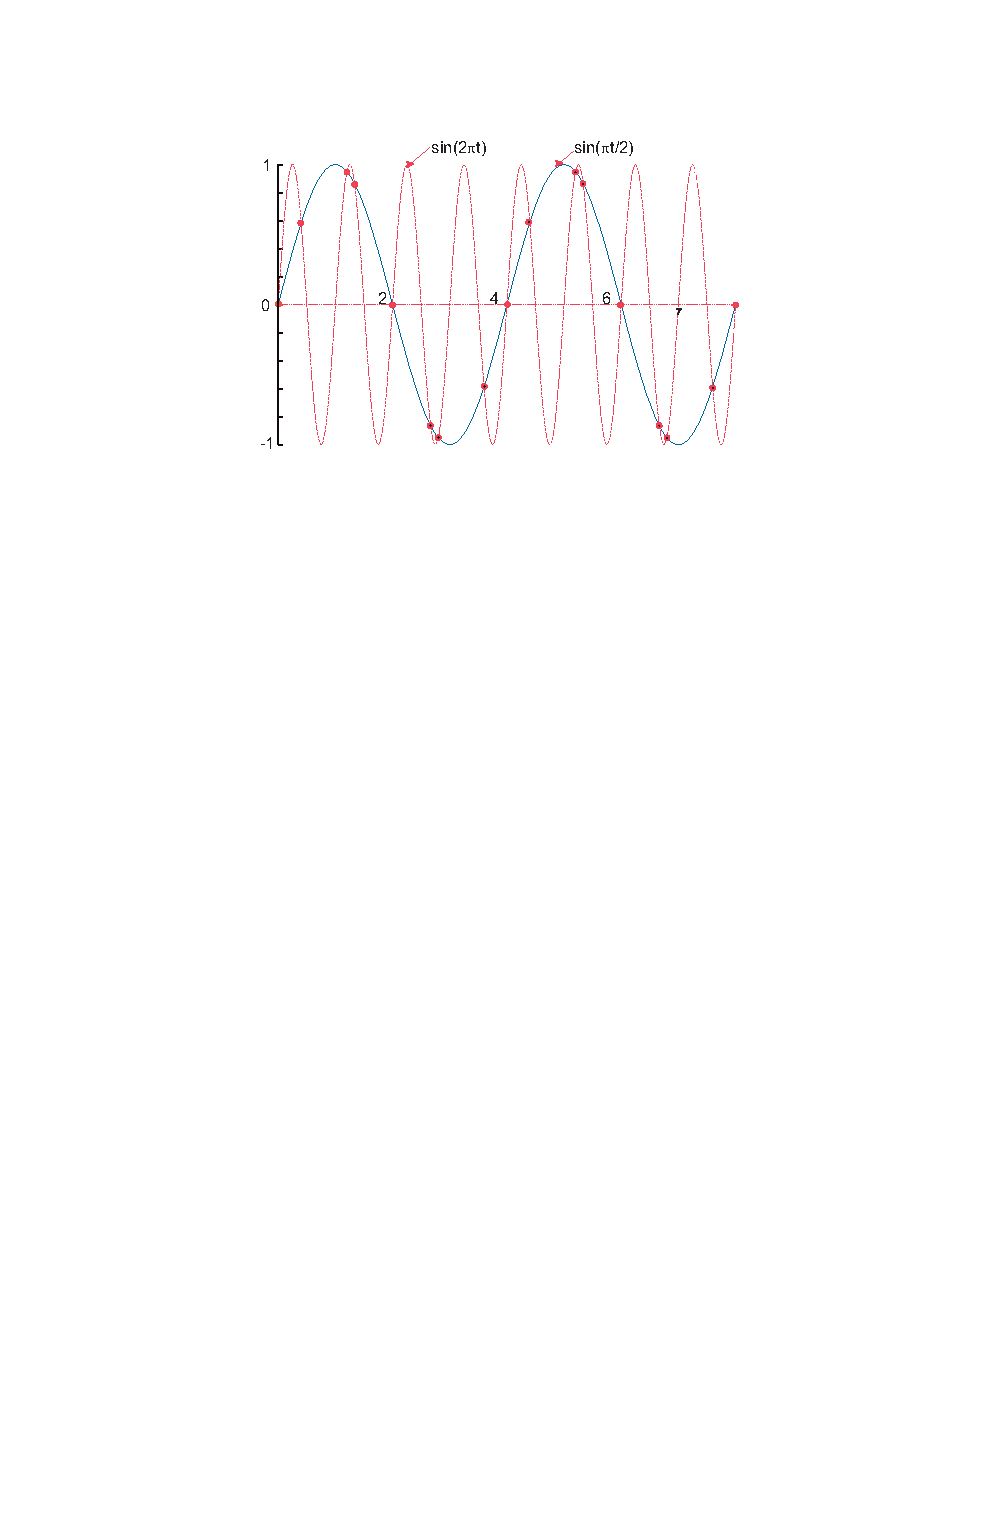
\includegraphics[width=0.9\columnwidth]{Aliasing.pdf}
  \end{figure}
  
\end{frame}

%-----------------------------------------------------------------------------------------

\begin{frame}%[fragile,shrink=15]
  \frametitle{Discrete Fourier Transforms (II)}

  The DFT algorithm results from evaluating the integral not from $1$ to $+1$ but rather from time $0$ to time $T$ over which the signal is measured, and from approximating the integration of the integral by computing a discrete sum:
  
  \begin{eqnarray}
    \hat{f}(\omega_n) &=& \frac{1}{\sqrt{2\pi}} \int_{-\infty}^{\infty} f(t)   e^{-i\omega_n t}   dt \\
                 &\simeq& \frac{1}{\sqrt{2\pi}} \int_{0}^{T}            f(t)   e^{-i\omega_n t}   dt \\
                 &\simeq& \frac{1}{\sqrt{2\pi}} \sum_{k=1}^{N}        h f(t_k) e^{-i\omega_n t_k} \qquad (h\equiv\mathrm{stepsize}) \\
                 &\simeq& \frac{h}{\sqrt{2\pi}} \sum_{k=1}^{N}          f_k    e^{-2\pi i k n/N}     \\
    \hat{f}_n \equiv \frac{\hat{f}(\omega_n)}{h} &=& \frac{1}{\sqrt{2\pi}} \sum_{k=1}^{N}  f_k  e^{-2\pi i k n/N}  
  \end{eqnarray}
  
\end{frame}

%-----------------------------------------------------------------------------------------

\begin{frame}%[fragile,shrink=15]
  \frametitle{Discrete Fourier Transforms (III)}

  We then need the inverse as well, which we can obtain with $d\omega \rightarrow 2\pi/Nh $ we invert the $\hat{f}_n $
      
  \begin{eqnarray}
    f_k &=& \frac{1}{\sqrt{2\pi}} \sum_{n=1}^{N} \frac{2\pi}{Nh}  \hat{f}_n  e^{i\omega_n t}  
  \end{eqnarray}
  
  Once we know the $N$ values of the transform $\hat{f}_n$, we can use this expression to evaluate $f(t)$ for any time $t$. The frequencies $\omega n$ are determined by the number of samples taken and by the total sampling time $T = N h$ as
  
  \begin{equation}
    \omega_n = n\frac{2\pi}{Nh}
  \end{equation}
  
  Clearly, the larger we make the time $T = Nh$ over which we sample the function, the smaller will be the frequency steps or resolution. Accordingly,if you want a smooth frequency spectrum, you need to have a small frequency step $2\pi/T$.
  
\end{frame}

%-----------------------------------------------------------------------------------------

\begin{frame}%[fragile,shrink=15]
  \frametitle{Discrete Fourier Transforms (IV)}

  Lastly, we can simplify this expression to yield a clear computational approach:
      
  \begin{eqnarray}
    f_k       &=& \frac{\sqrt{2\pi}}{N} \sum_{n=1}^{N} Z^{-nk}\hat{f}_{n} \qquad (Z=e^{-2\pi i/N}) \\
    \hat{f}_n &=& \frac{1}{\sqrt{2\pi}} \sum_{k=1}^{N} Z^{nk} f_k \qquad (n=0,1,\cdots,N) 
  \end{eqnarray}
  
  With this formulation, the computer needs to compute only powers of $Z$.
  
\end{frame}

%==========================================================================================
%==========================================================================================
\end{document}
